% The Hive in notation, after the owner's hand sketch: leads orange, workers green, wardens and
% tribunals red, structure in navy ink, on the site's diagram paper. Page 1 is the essay's figure
% (hive.svg), page 2 the front page's banner (hive-thumb.svg: 16:9, fewer and bigger glyphs).
% Redraw both with ./render.sh in this folder (XeLaTeX and dvisvgm, from TeX Live).
\documentclass[tikz,border=0pt]{standalone}
\usepackage{amsmath}
\usepackage{fontspec}
\usepackage{unicode-math}
\setmainfont{LibertinusSerif}[Extension=.otf, UprightFont=*-Regular, ItalicFont=*-Italic, BoldFont=*-Semibold]
\setmathfont{LibertinusMath-Regular.otf}
\usetikzlibrary{matrix,decorations.pathreplacing,calligraphy,arrows.meta,backgrounds,calc}

\definecolor{paper}{HTML}{FAF8F3}
\definecolor{ink}{HTML}{2A4470}
\definecolor{note}{HTML}{52607C}
\definecolor{lead}{HTML}{A6530F}
\definecolor{work}{HTML}{2E7443}
\definecolor{ward}{HTML}{A33A1E}
\definecolor{ghost}{HTML}{8F887C}

% A label in tracked capitals, like the site's own small labels.
\newcommand\caps[2][\footnotesize]{{#1\addfontfeatures{LetterSpace=9}\MakeUppercase{#2}}}
\newcommand\sep{\ $\cdot$\ }
\newcommand\La[1]{\textcolor{lead}{L_{#1}}}
\newcommand\Wo[1]{\textcolor{work}{W_{#1}}}
\newcommand\Wa[1]{\textcolor{ward}{\mathit{Wa}_{#1}}}
\newcommand\Tr[1]{\textcolor{ward}{\mathit{Tr}_{#1}}}

\tikzset{
  head/.style={text=ink, inner sep=1pt},
  note/.style={font=\itshape\small, text=note, align=left, inner sep=1pt},
  >={Stealth[length=4.5pt, width=3.5pt]},
  arr/.style={->, draw=ink, line width=0.55pt},
  brace/.style={decorate, decoration={calligraphic brace, amplitude=5pt}, line width=1pt, pen colour=ink},
  cell/.style={inner sep=1.5pt, text height=1.7ex, text depth=0.6ex},
  mat/.style={matrix of math nodes, left delimiter={[}, right delimiter={]}, row sep=2pt, column sep=8pt,
    nodes={cell, anchor=center}},
  list/.style={matrix of nodes, column sep=5pt, row sep=1pt, nodes={cell, anchor=base west}},
  every left delimiter/.style={xshift=1.5pt},
  every right delimiter/.style={xshift=-1.5pt},
}

\begin{document}

% ---------------------------------------------------------------- page 1: the essay's figure
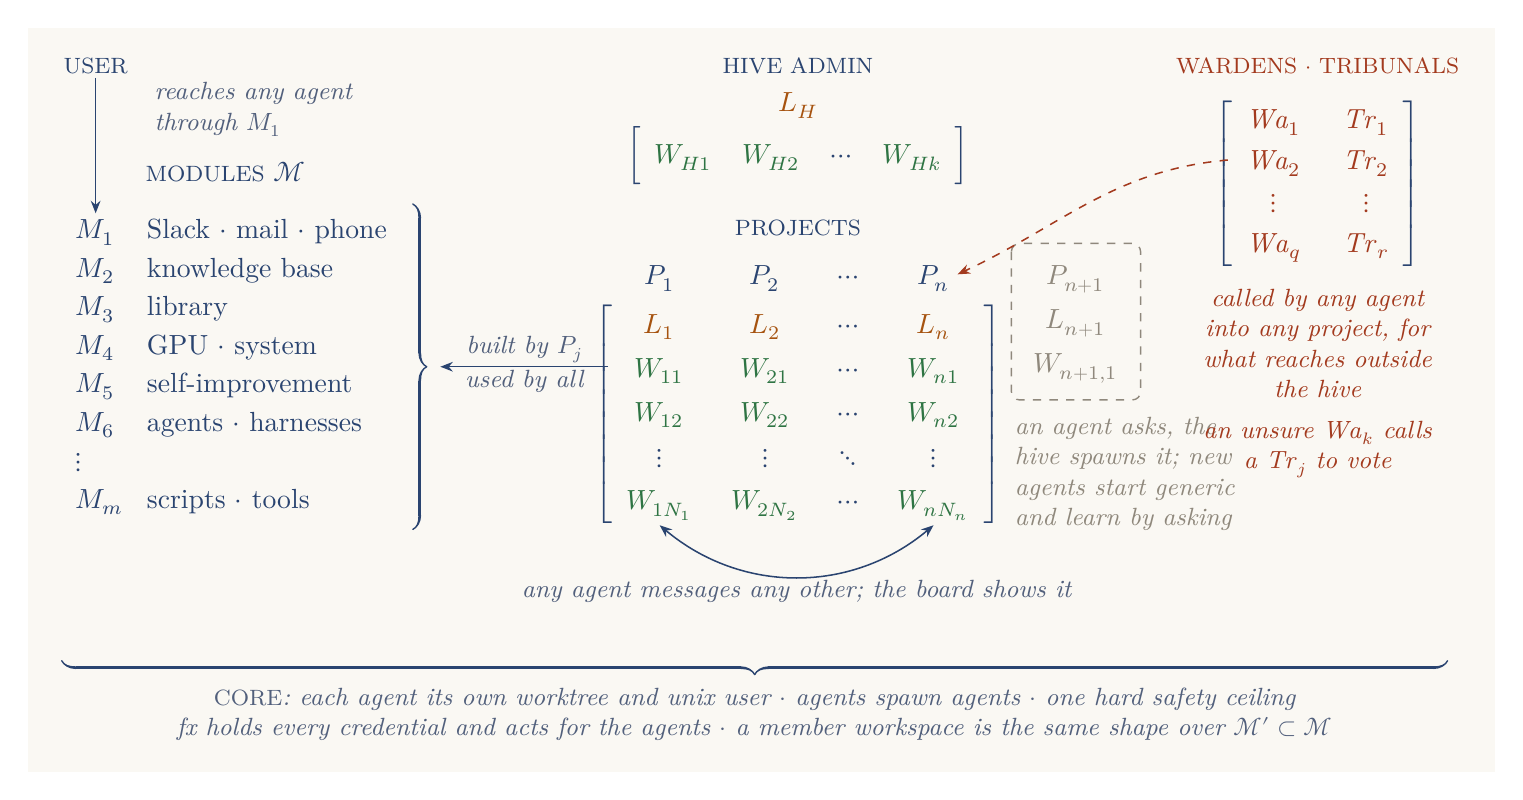
\begin{tikzpicture}[color=ink, line width=0.6pt, show background rectangle,
    background rectangle/.style={fill=paper, draw=none}, inner frame xsep=12pt, inner frame ysep=10pt]

% modules down the left, the user reaching any agent through M_1
\matrix (M) [list, anchor=north west] at (0.15,-1.75) {
  $M_1$ & Slack\sep{}mail\sep{}phone \\
  $M_2$ & knowledge base \\
  $M_3$ & library \\
  $M_4$ & GPU\sep{}system \\
  $M_5$ & self-improvement \\
  $M_6$ & agents\sep{}harnesses \\
  $\vdots$ & \\
  $M_m$ & scripts\sep{}tools \\
};
\node[head, anchor=base west] at ($(M-1-2.base west)+(0,0.72)$) {\caps{modules} $\mathcal{M}$};
\node[head] (U) at (M-1-1 |- 0,0) {\caps{user}};
\draw[arr] (U.south) -- (M-1-1.north);
\node[note, anchor=west] at ($(U.east)+(0.25,-0.55)$) {reaches any agent\\through $M_1$};

% hive admin, top centre
\node[head] at (9.5,0) {\caps{hive admin}};
\node at (9.5,-0.5) {$\La H$};
\matrix (H) [mat, anchor=north] at (9.5,-0.8) {
  \Wo{H1} & \Wo{H2} & \cdots & \Wo{Hk} \\
};

% projects: one column each, a lead over its workers
\node[head] at (9.5,-2.05) {\caps{projects}};
\matrix (P) [mat, anchor=north, row sep=3pt, column sep=11pt] at (9.5,-2.95) {
  \La1 & \La2 & \cdots & \La n \\
  \Wo{11} & \Wo{21} & \cdots & \Wo{n1} \\
  \Wo{12} & \Wo{22} & \cdots & \Wo{n2} \\
  \vdots & \vdots & \ddots & \vdots \\
  \Wo{1N_1} & \Wo{2N_2} & \cdots & \Wo{nN_n} \\
};
\foreach \j/\t in {1/P_1, 2/P_2, 3/\cdots, 4/P_n}
  \node[anchor=base, inner sep=1pt] (Ph\j) at ($(P-1-\j.base)+(0,0.62)$) {$\t$};

% the next project, asked for by an agent
\matrix (G) [matrix of math nodes, anchor=north west, row sep=3pt, nodes={cell, text=ghost}]
    at ($(P.north east)+(0.45,0.62)$) {
  P_{n+1} \\ L_{n+1} \\ W_{n+1,1} \\
};
\draw[ghost, dashed, line width=0.5pt, rounded corners=3pt]
  ($(G.north west)+(-0.1,0.08)$) rectangle ($(G.south east)+(0.1,-0.08)$);
\node[note, anchor=north west, text=ghost] at ($(G.south west)+(-0.1,-0.25)$)
  {an agent asks, the\\hive spawns it; new\\agents start generic\\and learn by asking};

% modules are built by projects and used by every agent
\draw[brace] ($(M.north east)+(0.15,0)$) -- ($(M.south east)+(0.15,0)$);
\draw[arr] ($(P.west |- M.east)+(-0.05,0)$) -- node[note, above] {built by $P_j$} node[note, below] {used by all}
  ($(M.east)+(0.5,0)$);

% wardens and tribunals, top right
\node[head, text=ward] at (16.1,0) {\caps{wardens\sep{}tribunals}};
\matrix (R) [mat, color=ward, anchor=north, column sep=12pt] at (16.1,-0.35) {
  \Wa1 & \Tr1 \\
  \Wa2 & \Tr2 \\
  \vdots & \vdots \\
  \Wa q & \Tr r \\
};
\node[note, text=ward, align=center, anchor=north] (Rn) at ($(R.south)+(0,-0.15)$)
  {called by any agent\\into any project, for\\what reaches outside\\the hive};
\node[note, text=ward, align=center, anchor=north] at ($(Rn.south)+(0,-0.2)$) {an unsure $\Wa{k}$ calls\\a $\Tr{j}$ to vote};
\draw[arr, draw=ward, dashed] ($(R.west)+(-0.05,0.3)$) to[out=185, in=25] ($(Ph4.east)+(0.05,0.05)$);

% any agent messages any other
\draw[<->, draw=ink, line width=0.55pt]
  ($(P-5-1.south)+(0,-0.05)$) to[out=-40, in=-140]
  node[note, below] {any agent messages any other; the board shows it} ($(P-5-4.south)+(0,-0.05)$);

% everything above runs on the core
\draw[brace] (17.75,-7.55) -- (0.15,-7.55);
\node[note, anchor=north, align=center] at (8.95,-7.85)
  {\textup{\caps{core}}: each agent its own worktree and unix user\sep{}agents spawn agents\sep{}one hard safety ceiling\\
   \textit{fx} holds every credential and acts for the agents\sep{}a member workspace is the same shape over $\mathcal{M}'\subset\mathcal{M}$};
\end{tikzpicture}

% ---------------------------------------------------------------- page 2: the banner, 16:9
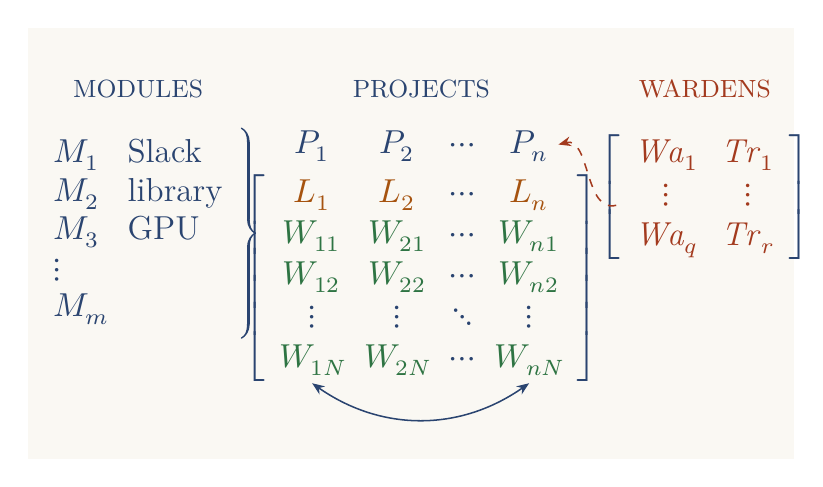
\begin{tikzpicture}[color=ink, line width=0.6pt, every node/.style={font=\large}]
\useasboundingbox[fill=paper] (0,0) rectangle (9.737,5.477);

\matrix (M) [list, anchor=north west, column sep=3pt] at (0.15,4.2) {
  $M_1$ & Slack \\
  $M_2$ & library \\
  $M_3$ & GPU \\
  $\vdots$ & \\
  $M_m$ & \\
};
\node[head] at (M.north |- 0,4.7) {\caps[\small]{modules}};
\draw[brace] ($(M.north east)+(0.06,0)$) -- ($(M.south east)+(0.06,0)$);

\node[head] at (5.0,4.7) {\caps[\small]{projects}};
\matrix (P) [mat, anchor=north, row sep=2pt, column sep=4pt] at (5.0,3.7) {
  \La1 & \La2 & \cdots & \La n \\
  \Wo{11} & \Wo{21} & \cdots & \Wo{n1} \\
  \Wo{12} & \Wo{22} & \cdots & \Wo{n2} \\
  \vdots & \vdots & \ddots & \vdots \\
  \Wo{1N} & \Wo{2N} & \cdots & \Wo{nN} \\
};
\foreach \j/\t in {1/P_1, 2/P_2, 3/\cdots, 4/P_n}
  \node[anchor=base, inner sep=1pt] (Ph\j) at ($(P-1-\j.base)+(0,0.62)$) {$\t$};
\draw[<->, line width=0.55pt] ($(P-5-1.south)+(0,-0.05)$) to[out=-35, in=-145] ($(P-5-4.south)+(0,-0.05)$);

\node[head, text=ward] at (8.6,4.7) {\caps[\small]{wardens}};
\matrix (R) [mat, color=ward, anchor=north, column sep=5pt] at (8.6,4.2) {
  \Wa1 & \Tr1 \\
  \vdots & \vdots \\
  \Wa q & \Tr r \\
};
\draw[arr, draw=ward, dashed] ($(R.west)+(-0.05,-0.1)$) to[out=195, in=15] ($(Ph4.east)+(0.08,0.02)$);
\end{tikzpicture}

\end{document}
